\chapter{Main Part of Code}
Our models are established based on language Python. In this appendix, we list the main part of our codes, which includes seven components:

1) Model preparation: Read order books and message books data of five stocks into python environment. Build features and responses based on different time interval.

2) Data split: Divide the features and responses data into training data and testing data based on the ratio of nine to one.

3) Two-class problem: Create binary classification models( predicting the future ask-low case of LOBs), which include logistic regression, lasso regression, ridge regression, support vector machine, decision tree, random forest, and AdaBoost.

4) Multi-class problem: Create binary classification models, which include logistic regression, lasso regression, ridge regression, support vector machine, decision tree, random forest, and AdaBoost, by use of one vs. one and one vs. rest methods.

5) PnL calculation: Design a simple trading strategy and calculate the PnL based on ensemble predicting models.

6) Order book structure plotting: Plot the structures of LOBs which include volume, size, snapshot and relative depth of LOBs.

7) Statistical properties of LOBs plotting: Plot the statistical properties of LOBs which contain distribution, average shape, intraday seasonality of LOBs.

The python code can be found in my github:\\
https://github.com/wangjian790/Python/blob/master/research/
% 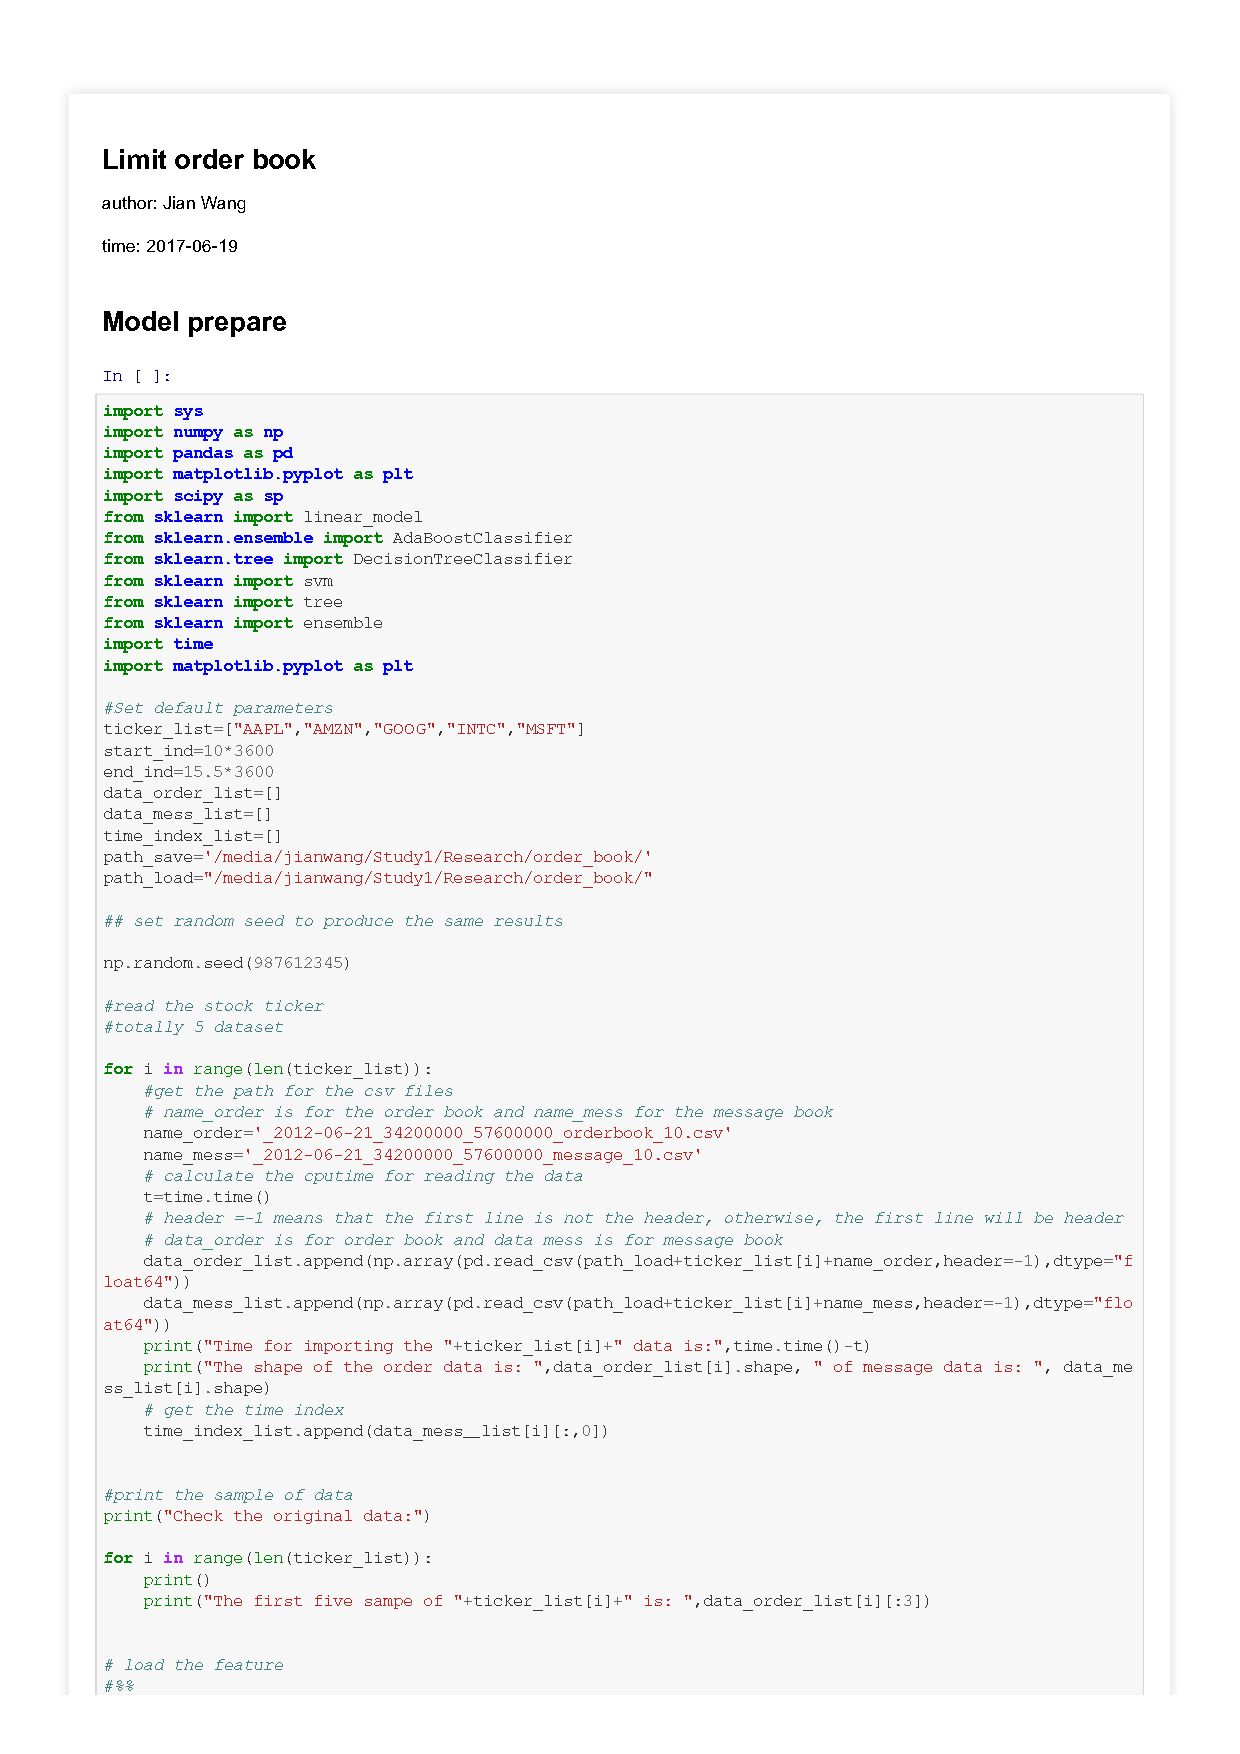
\includepdf[pages=1-,pagecommand={},offset=0.5cm 0cm,scale=0.85]{order_book_summary.pdf}